\documentclass[letterpaper, 12pt]{article}
\usepackage{graphicx}
\usepackage{amsmath}
\usepackage{float}

\graphicspath{{./pics/}}
\begin{document}
\title{6.013 Final project Report}
\author{Andres Erbsen, Justin Graves, Dimitris Koutentakis}
\date{\today}
\maketitle
\vspace{5mm}
\tableofcontents
\clearpage
\section{Abstract}
From 6.013 we learned that transmission lines can resonate at certain frequencies and create standing waves due to the geometry and what happens at the boundaries of the lines. We also learned that as the boundary geometry changes the electromagnetic fields inside the boundaries also change. From this idea it is reasonable to come to the conclusion that you should be able to "select" which electromagnetic waves can pass through the transmission by designing a specific geometry for the intersted electromagnetic wave.

\section {Introduction}
\section{Approach}
In order to design our filters, we had to apply some of the basic knowledge we acquired in the lectures towards the end of the semester. More specifically, we had to apply knowledge regarding transmission line resonators as well as smith charts and stubs.
\\
By calculating the dimensions for our given substrate and target frequencies we were able to build the filters desired. The filters that we ended up building are:
\begin{itemize}
    \item A short-short half wave resonator built with the dimensions of the original substrate board,
    \item A short-short half wave resonator for $f=2.4 GHz$,
    \item A single stub band-stop resonator, and
    \item A multiple stub band pass approximation filter
\end{itemize}
\subsection{Short-short half wave resonator}
For the first short-short half-wave resonator, we used the dimensions of the original board given. More specifically, we used the length of the board, $D=7.7cm$ and $\delta$ very small in order to maximize our $Q$. Given the substrate and the width of the board, we calculated that this filter would work optimally for a frequency of $f=1.28 GHz$
\begin{align*}
    D=7.7cm &\Rightarrow \frac{\lambda_n}{2}=7.7cm \\
    \lambda_0=7.7cm\cdot2\cdot\sqrt{2.33}&\Rightarrow \lambda_0=23.5cm \\
    f=\frac{3\cdot10^{8}}{23.5\cdot10^{-2}} &\Rightarrow f=1.277 GHz
\end{align*}

\begin{figure}[H]
    \centering
    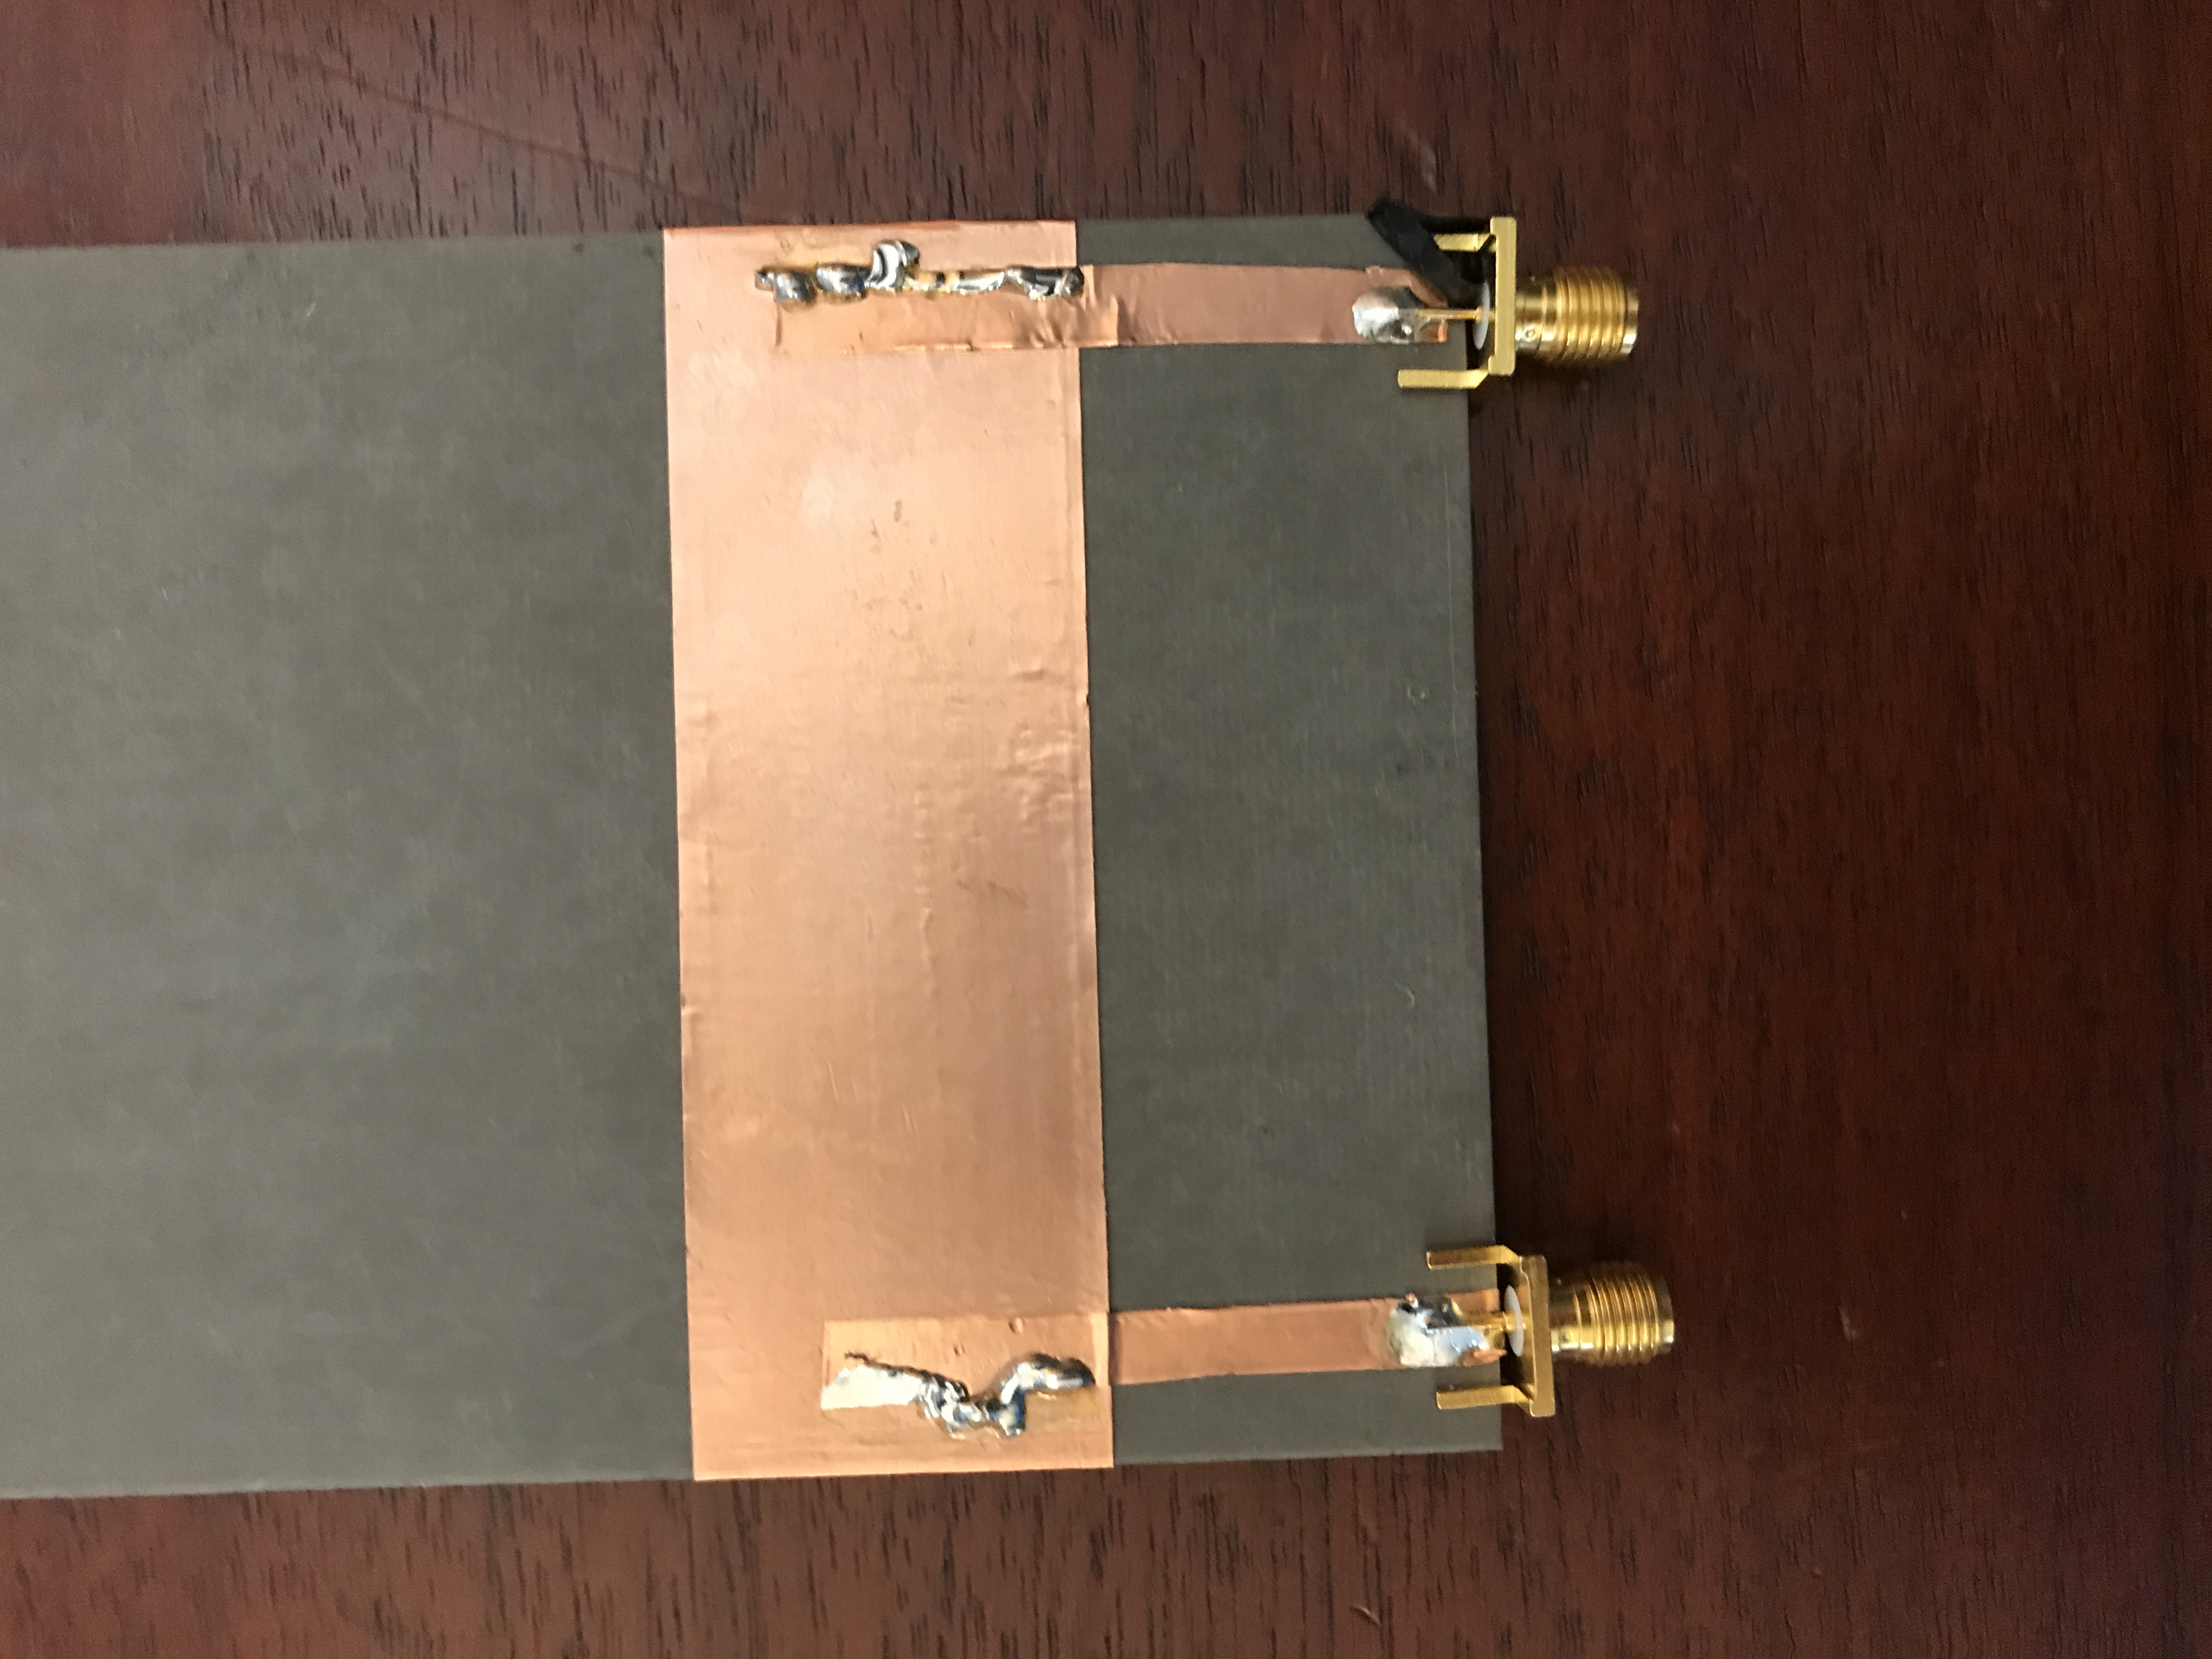
\includegraphics[width=0.8\textwidth, angle = 270]{filter1}
    \caption{Original width half-wave resonator filter}
\end{figure}
% \clearpage
\subsection{Short-short 2.4 GHz resonator}
In order to build a filter aimed at our radar's working frequency, we had to design and build a filter that would work at around 2.4 GHz. The calculations we made can be seen below:
\begin{equation*}
\left.
\begin{aligned}
    D&=\frac{m\cdot\lambda_n}{2} \\
    \lambda_n&=\frac{\lambda_0}{n}\\
    m&=1 \\
    \epsilon_r&=2.33 \\
    \mu_r&=1
\end{aligned}
\right \}
\Longrightarrow
D=0.0409m
\end{equation*}
After cutting the substrate boards at the calculated dimensions, we had the following filter:

\begin{figure}[H]
    \centering
    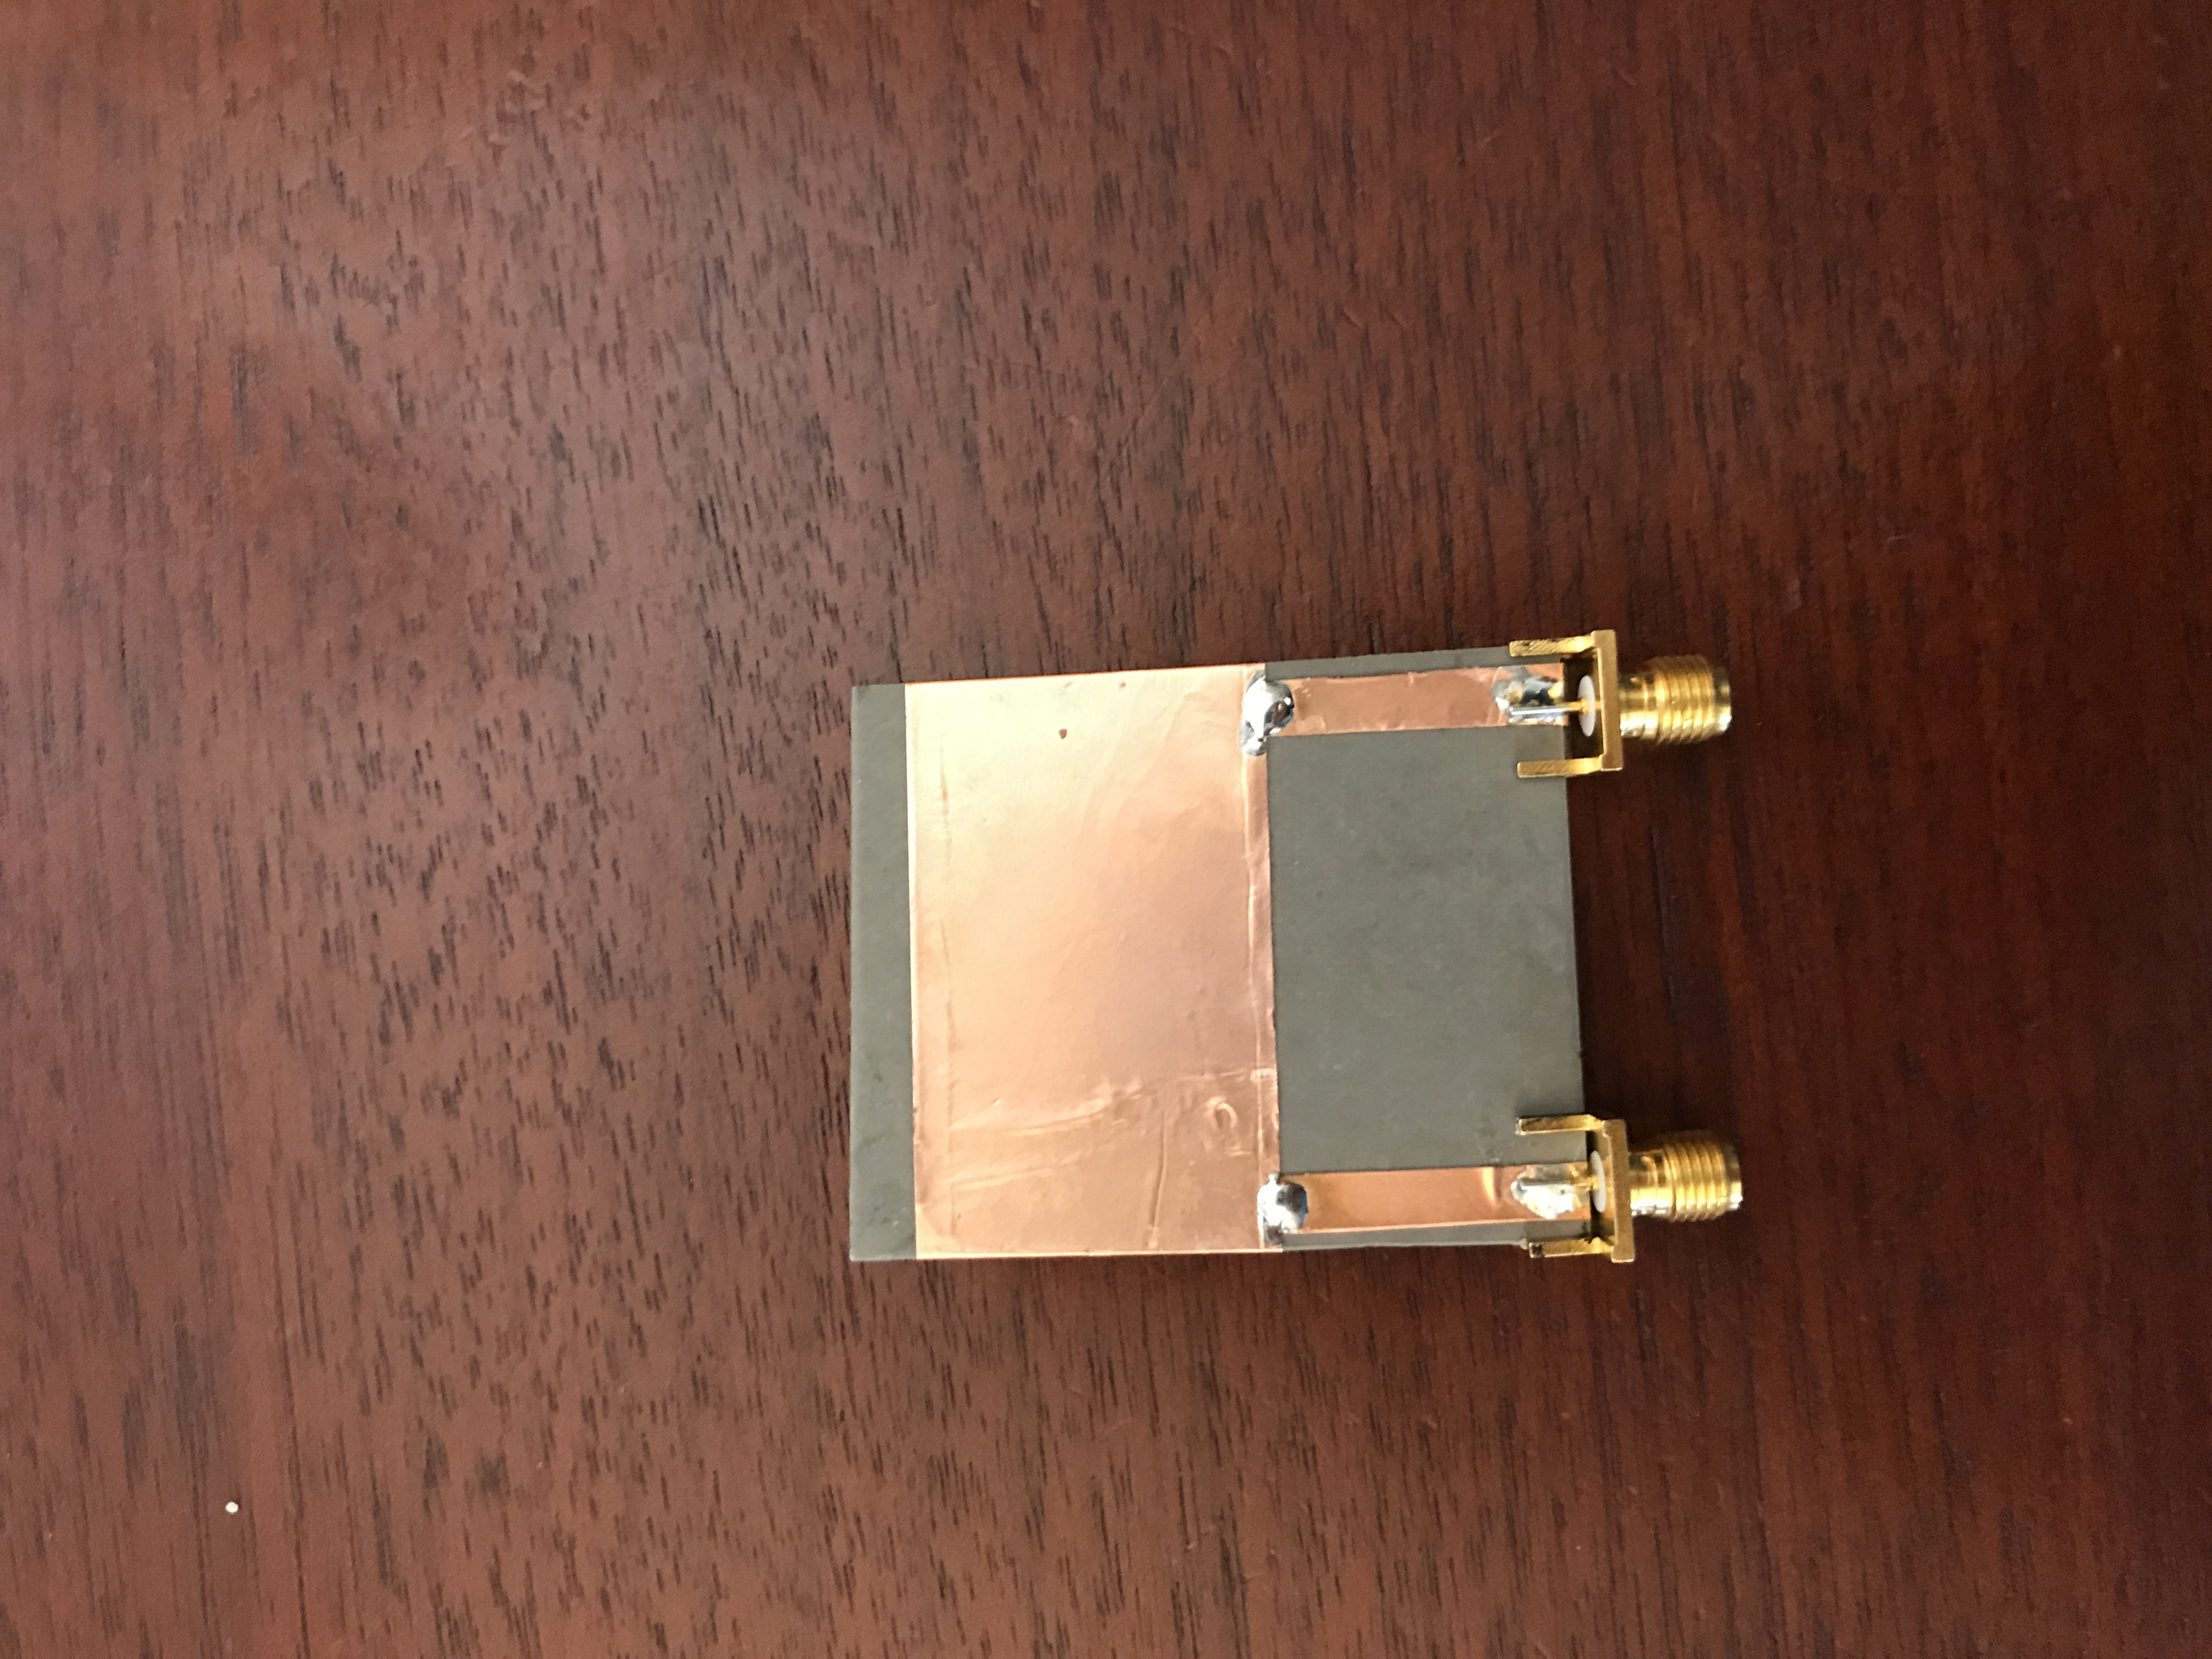
\includegraphics[width=0.8\textwidth, angle = 270]{filter2}
    \caption{2.4GHz half-wave resonator filter}
\end{figure}

\subsection{Single stub band-stop filter}
describe
\subsection{multiple stub band-pass filter}
describes
\section{Measurements}

\subsection{Short-short half wave resonator}
\begin{figure}
    \centering
    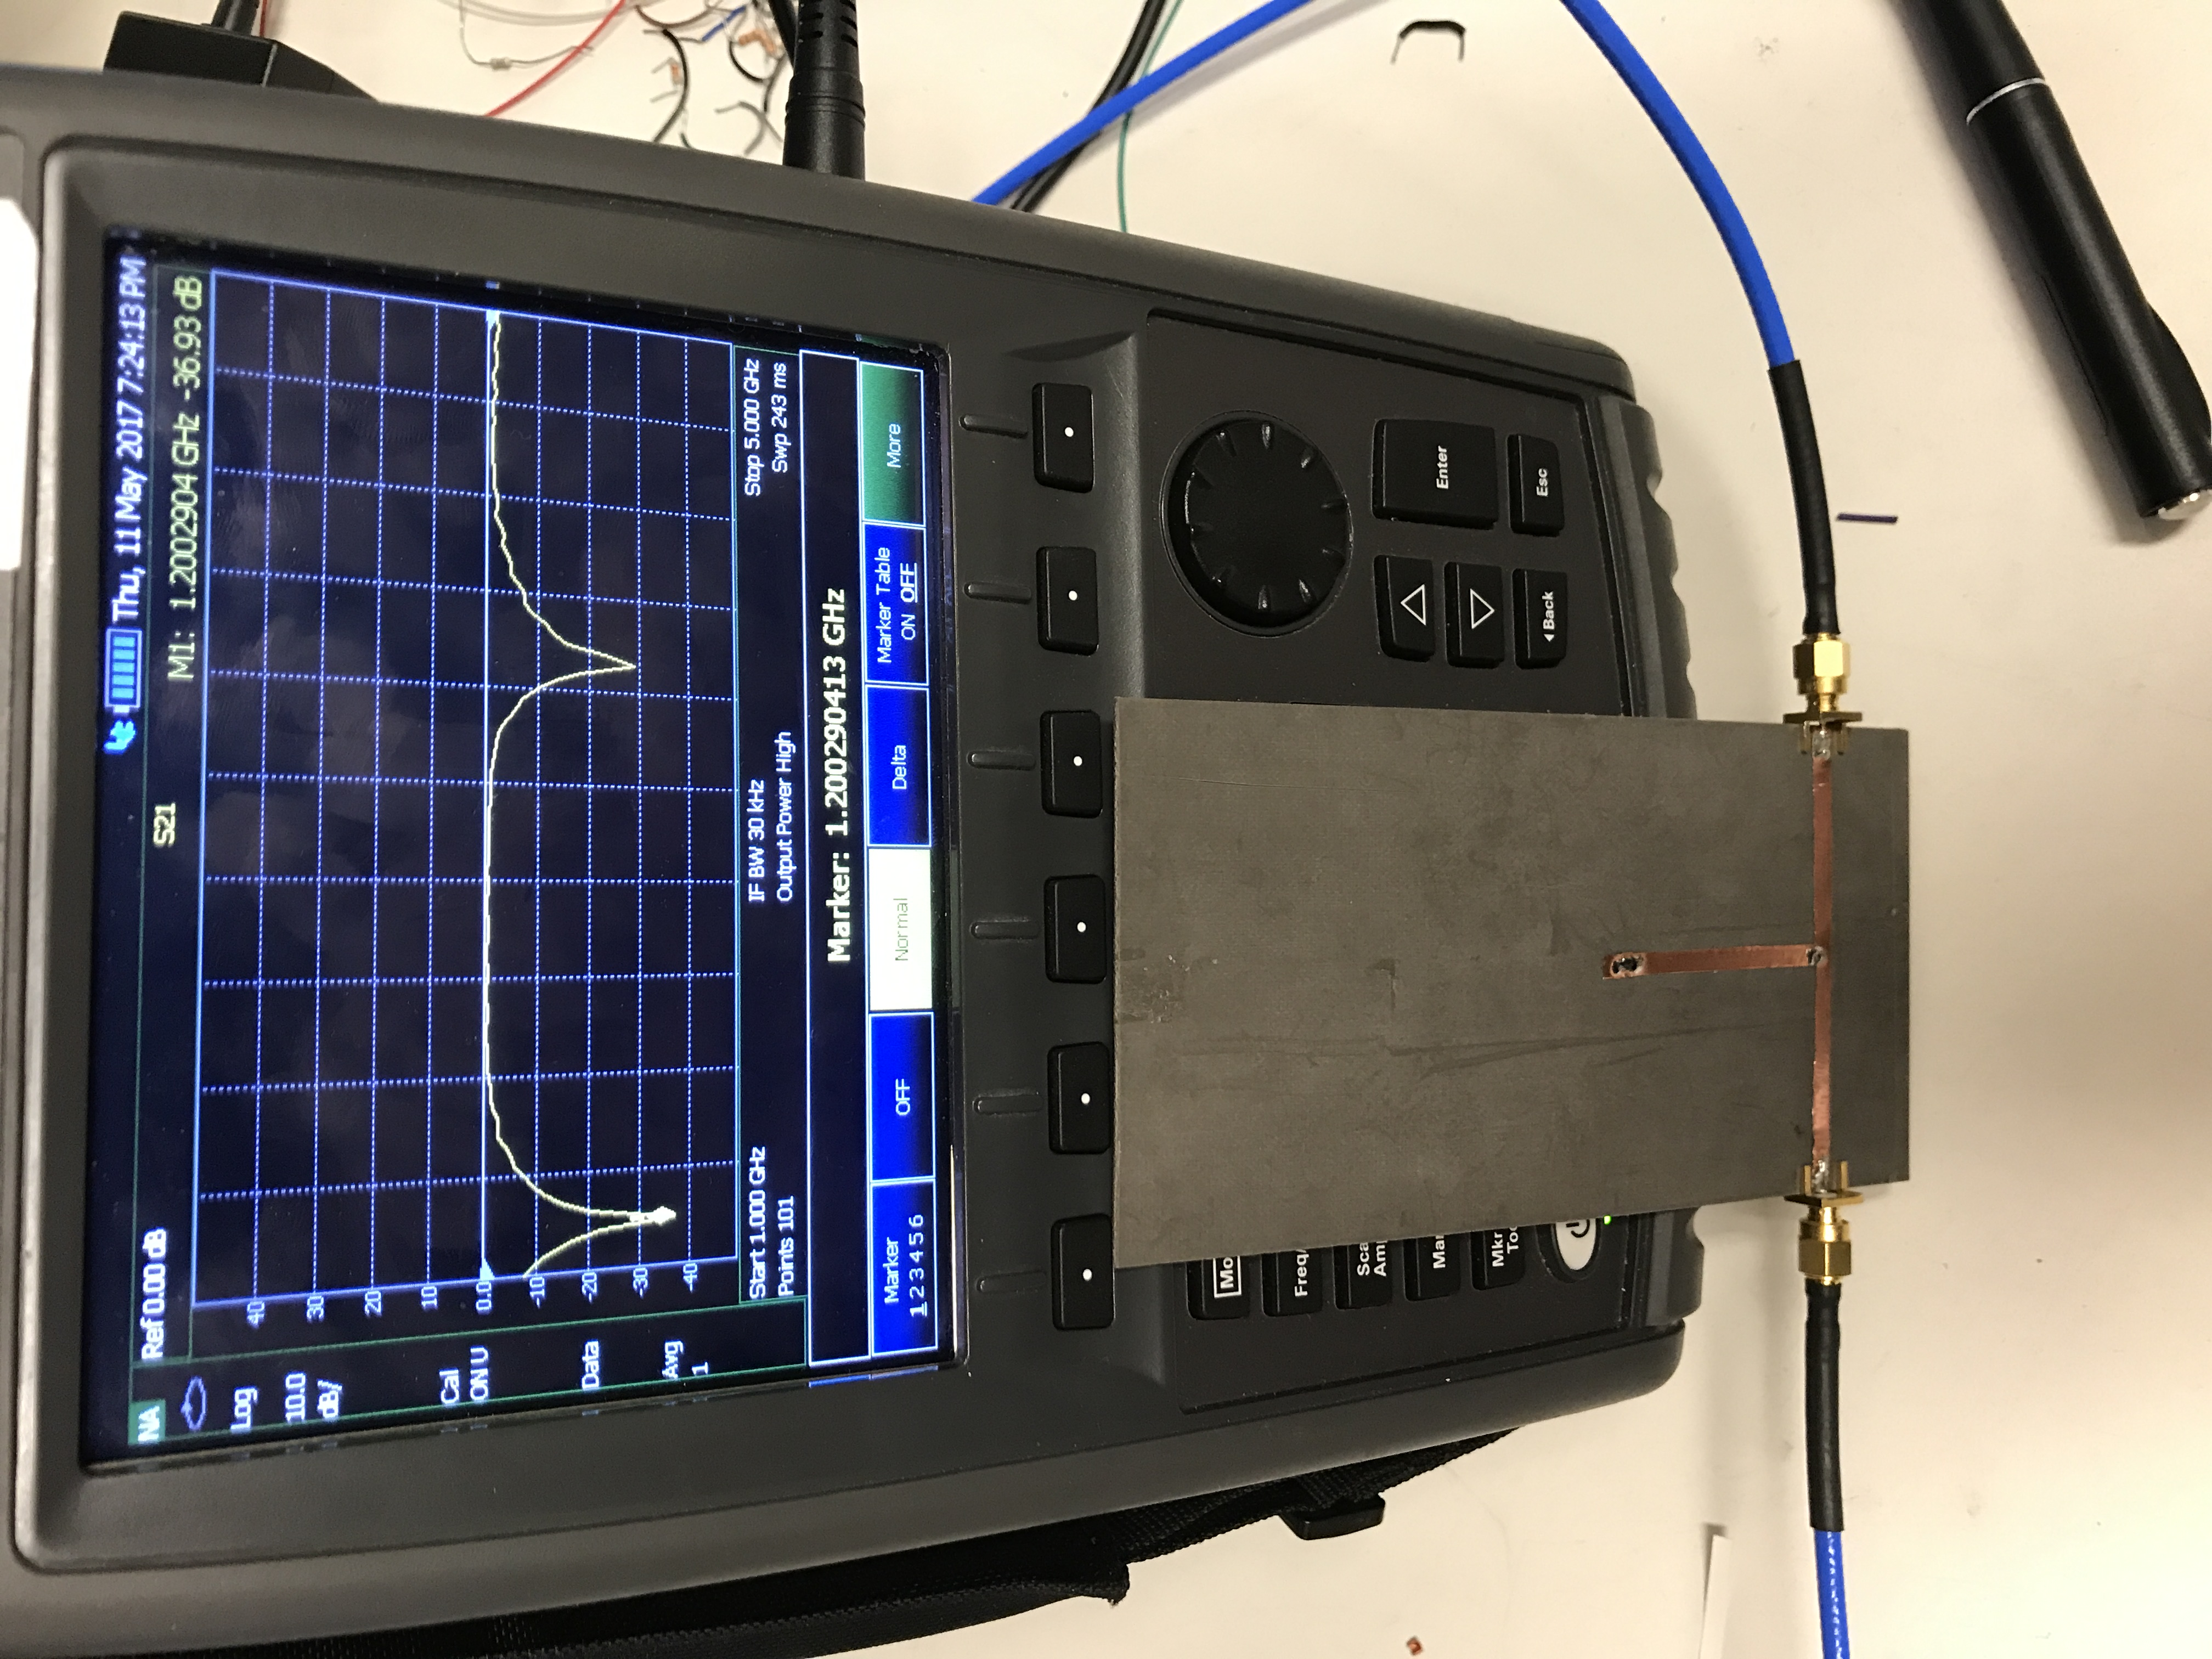
\includegraphics[width=0.8\textwidth, angle=270]{1stub}
    \caption {single stub measurements}
\end{figure}
\subsection{Short-short 2.4 GHz resonator}


\subsection{Single stub band-stop filter}
describe
\subsection{multiple stub band-pass filter}
describes

\section{Discussion}
describe
\end{document}

